\documentclass[tikz]{standalone}
\usepackage{pgfplots}
\pgfplotsset{compat=1.15}
\usepackage{mathrsfs}
\usetikzlibrary{arrows,calc}
\usepackage{tkz-euclide}
\pagestyle{empty}

\definecolor{AngleClr}{rgb}{0,0.39215686274509803,0}
\definecolor{ShapeClr}{rgb}{0.6,0.2,0}

\begin{document}

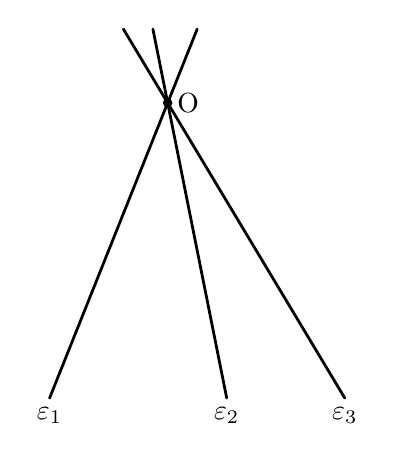
\begin{tikzpicture}[scale=.75]
\tkzSetUpLine[line width=1pt,color=black]
\tkzSetUpPoint[fill=black]

\tkzDefPoints{2/5/O,0/0/A,3/0/B,5/0/C}

% Define the parallel lines.
\tkzDefPoints{-0.2/2.6/D1A,5.2/2.6/D1B}
\tkzDefPoints{-0.2/1/D2A,5.2/1/D2B}

\tkzInterLL(D1A,D1B)(O,A) \tkzGetPoint{I1}
\tkzInterLL(D1A,D1B)(O,B) \tkzGetPoint{I2}
\tkzInterLL(D1A,D1B)(O,C) \tkzGetPoint{I3}

\tkzInterLL(D2A,D2B)(O,A) \tkzGetPoint{J1}
\tkzInterLL(D2A,D2B)(O,B) \tkzGetPoint{J2}
\tkzInterLL(D2A,D2B)(O,C) \tkzGetPoint{J3}



\tkzDrawSegments[color=black,add=0.25 and 0](O,A O,B O,C)
% \tkzDrawSegments[color=black](D1A,D1B)
% \tkzDrawSegments[color=black](D2A,D2B)

\tkzDrawPoints[size=3](O)

\tkzLabelPoint[right](O){$\rm O$}

\tkzLabelPoint[below](A){$\varepsilon_1$}
\tkzLabelPoint[below](B){$\varepsilon_2$}
\tkzLabelPoint[below](C){$\varepsilon_3$}


% \tkzLabelPoint[right](D1B){$\delta_1$}
% \tkzLabelPoint[right](D2B){$\delta_2$}

\end{tikzpicture}
\end{document}
